\documentclass[tikz,border=8pt]{standalone}
\usepackage{tikz}
\usetikzlibrary{shapes,arrows,positioning}
\tikzstyle{proc}=[rectangle,draw,rounded corners,fill=blue!10,align=center,minimum width=3.4cm,minimum height=0.9cm,font=\small]
\tikzstyle{dec}=[diamond,draw,fill=green!10,align=center,aspect=2,font=\small]
\tikzstyle{term}=[rectangle,draw,rounded corners=8pt,fill=gray!15,align=center,minimum width=2.6cm,minimum height=0.9cm,font=\small\bfseries]
\tikzstyle{arr}=[->,thick]
\begin{document}
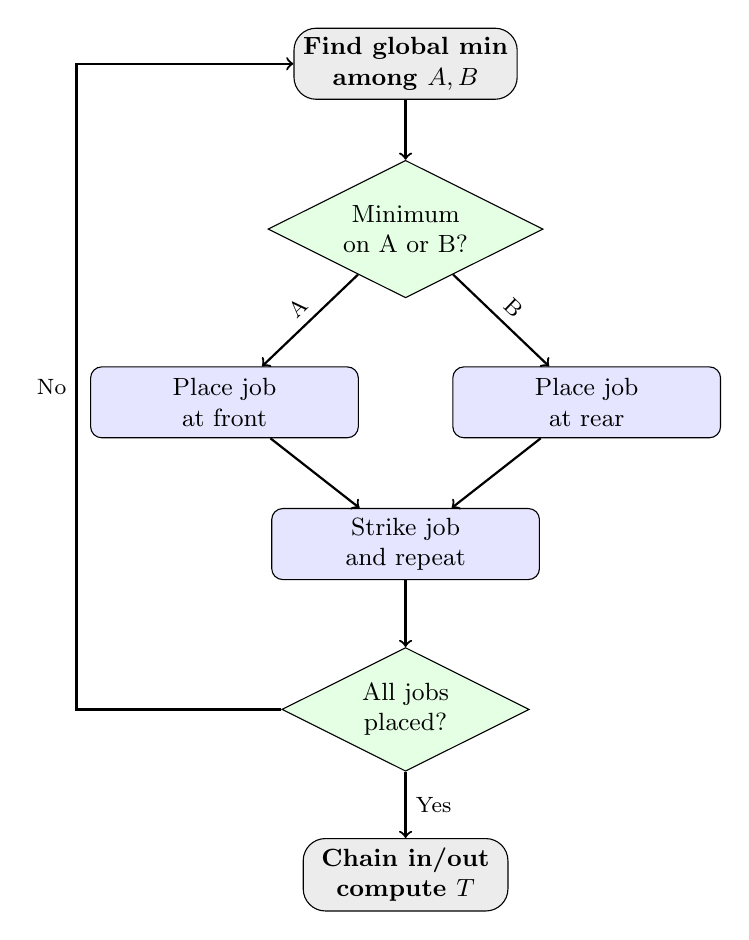
\begin{tikzpicture}[node distance=1.7cm]
\node[term] (A) {Find global min\\among $A,B$};
\node[dec, below of=A, yshift=-0.4cm] (B) {Minimum\\on A or B?};
\node[proc, below of=B, xshift=-2.3cm, yshift=-0.5cm] (C) {Place job\\at front};
\node[proc, below of=B, xshift=2.3cm, yshift=-0.5cm] (D) {Place job\\at rear};
\node[proc, below of=B, yshift=-2.3cm] (E) {Strike job\\and repeat};
\node[dec, below of=E, yshift=-0.4cm] (F) {All jobs\\placed?};
\node[term, below of=F, yshift=-0.4cm] (G) {Chain in/out\\compute $T$};
\draw[arr] (A) -- (B);
\draw[arr] (B) -- node[above,sloped,font=\footnotesize]{A} (C);
\draw[arr] (B) -- node[above,sloped,font=\footnotesize]{B} (D);
\draw[arr] (C) -- (E);
\draw[arr] (D) -- (E);
\draw[arr] (E) -- (F);
\draw[arr] (F) -- node[right,font=\footnotesize]{Yes} (G);
\draw[arr] (F.west) -- ++(-2.6,0) |- node[left,font=\footnotesize,pos=0.25]{No} (A.west);
\end{tikzpicture}
\end{document}
